% File hicss51.tex
%%
%% Based on the style files for ACL 2015 by 
%% car@ir.hit.edu.cn, gdzhou@suda.edu.cn


\documentclass[10pt]{article}
\usepackage[letterpaper]{geometry}
\usepackage{hicss51}
\usepackage{times}
\usepackage[none]{hyphenat}
\usepackage{url}
\usepackage{latexsym}
%\usepackage{minted}
\usepackage{indentfirst}
\usepackage{graphicx}
%\graphicspath{{images/}}
\usepackage{wrapfig}
\usepackage{todonotes}
\usepackage{hyperref}
\usepackage[utf8]{inputenc}
\newcommand{\sansserifformat}[1]{\fontfamily{cmss}{ #1}}%

%\setlength\titlebox{5cm}


% You can expand the titlebox if you need extra space
% to show all the authors. Please do not make the title box
% smaller than 5cm (the original size).



\title{Open Source Intelligence - Development of a Trend Radar utilizing a Systematic Literature Review}

\author{Franz Kayser \\
  ESG \\
  {\underline{ franz.kayser@esg.de}} \\\And
  Thomas Mayer \\
  ESG  \\
  {\underline{ thomas3.mayer@esg.de} }\\\And 
  Michael Bücker \\
  FH Münster -- University of Applied Sciences\\
  {\underline{michael.buecker@fh-muenster.de}} \\}

\date{}

\begin{document}
\maketitle
\begin{abstract}


    Open Source Intelligence (OSINT) is currently experiencing an intensive discourse,
    heightened since the Russian invasion of Ukraine. However, despite numerous attempts
    at standardized definitions, the intelligence discipline remains ambiguous. This paper
    introduces a practice-validated OSINT trend radar, categorizing technologies by maturity,
    intelligence cycle phase, and use case. Serving as a profound knowledge base and tool for
    identifying research gaps, the radar emerges from a structured design process. Sixty
    studies underwent categorization and validation through expert interviews,
    revealing the absence of a comprehensive, automated third-generation OSINT
    system in Germany. Technological gaps, especially in the planning, direction,
    dissemination, and integration phases, are evident. Although intelligent support
    technologies were identified, practical implementation lags behind theory. The human
    factor therefore remains central to the OSINT process. Future research should thus
    prioritize developing applications for underserved phases, probing reasons for limited
    widespread implementation of proven applications, with emphasis on legal, ethical,
    political, and social parameters.


\end{abstract}

\section{Introduction}

OSINT is a currently more debated research field than ever before. Obtaining intelligence
from publicly available data \cite{DosPassos.2017} has become undeniably important since the
Russian invasion of Ukraine in 2022. The real-time analysis of social media in particular has
brought highly relevant findings to light \cite{Hatfield.2023, SmithBoyle.24.07.2023}.
However, OSINT is not a new technique \cite{PastorGalindo.2019, Schaurer.2010}. However, despite
numerous attempts to define OSINT (e.g. \cite{Hwang.2022, PastorGalindo.2020, Yogish.2021}),
the concept remains controversial to this day \cite{Ghioni.2023, Ish.2022,Williams.2018}.
This is not least due to the fact that every definition of OSINT is subject to the advances
in computer and data sciences, which continuously produce improvements in (intelligent)
collection and analysis possibilities \cite{Ghioni.2023, Williams.2018}. In addition, this is
accompanied by numerous new open means of communication, which have caused a veritable
"information explosion"\cite{DosPassos.2017, Hwang.2022, Yogish.2021}.
Data sources that were originally reserved for the defense and intelligence services are
now also publicly accessible \cite{Hwang.2022, Williams.2018}. The understanding of
intelligence thus changed completely \cite{Dokman.2020}.

To date, there has been a lack of decisive, fundamental scientific publications to penetrate
the subject area \cite{HerreraCubides.2020} and address its rapid
developments \cite{Ghioni.2023, Williams.2018}. In particular, there is a shortage of
studies that identify the technologies behind OSINT and determine their characteristics.
The question of whether "third generation" OSINT systems in the sense of
robust, autonomous \cite{PastorGalindo.2019, PastorGalindo.2020} already exist
has not yet been clarified \cite{Ghioni.2023, PastorGalindo.2020,Yogish.2021}.
Moreover, the majority of studies focus exclusively on analyzing the OSINT trend area "cyber
security" \cite{Hwang.2022, PastorGalindo.2019, Yogish.2021}. The literature thus failed to
cover the topic in its entirety. Important application scenarios ("use cases") of OSINT have
therefore not yet been taken into account in research \cite{AlKilani.2021, Dokman.2020, Ghioni.2023}.
In addition, supplementary qualitative field research is absent to contrast theory with
the corresponding practical implementation. Although OSINT has a major impact on topics
such as security and defense, there is a lack of insight into these sectors \cite{HerreraCubides.2020, PastorGalindo.2019}.
This paper is hence dedicated to answer the research question:
\textit{How can the current trends in OSINT in the form of the technologies used and their
    characteristics, in particular the maturity level and the use case, be presented in a
    trend radar and validated by experts within the security sector?}

The aim thereby is to identify the technologies used in OSINT applications and to present
them systematically in a trend radar, according to their characteristics. Through expert
interviews, trends will then be validated. In this way, a well-founded knowledge base will
be compiled, and practice-relevant research gaps will be identified for a coordinated examination
of the research field. The study thereby follows the "Design Science Research Model" (DSRM)
\cite{Peffers.2007}.  First, the relevant literature on OSINT will be analyzed and classified
through a systematic literature review \cite{Webster.2002}. Second, the OSINT technologies and
their characteristics identified will be visualized in the form of a trend radar. The radar
will then be validated using systematizing interviews \cite{Bogner.2014} conducted with
experts in the security sector. Finally, the interviews will be evaluated using a
qualitative content analysis [21].


\section{Theoretical Background}
The domain of OSINT is continuously expanding due to the ongoing development of improved
collecting and analysis possibilities \cite{AlKilani.2021, Ghioni.2023, Williams.2018}. In
addition, the new means and methods of communication associated with advances in information
and communication technology have turned OSINT into a complex discipline
\cite{AlKilani.2021, Benes.2013, Chen.2012, Williams.2018}. OSINT and its
components are therefore defined in detail hereinafter.

\subsection{Open Source Intelligence (OSINT)}

One of the earliest and still frequently referenced definitions \cite{DosPassos.2017}
was published by NATO in 2001. OSINT according to this definition is information that has been
deliberately discovered, discriminated, distilled, and disseminated to a select audience,
[...], in order to address a specific question. OSINT, [...] thus applies the proven
process of intelligence to the broad diversity of open sources [...] and creates
intelligence [23]. However, today the discipline is no longer seen as a purely governmental
matter. Private research institutions and organizations \cite{Bohm.2021,Mercado.2005} are
also massively driving the development of such systems, e.g. for competitive analyses or marketing activities
\cite{AlKilani.2021, Dokman.2020,Ghioni.2023}. The focus is thereby shifting to
developing OSINT into a robust, autonomous solution [4,8,9].

\subsection{Open Source Data (OSD)}

The starting point for all OSINT activities is data. Data forms the basis of the
analysis and the conclusions derived from it \cite{Gibson.2016}. In this context, OSD
refers to non-processed \cite{DosPassos.2017}, general raw data that is openly available
\cite{Burke.2007} as well as legally and ethically accessible
\cite{Schaurer.2010, NorthAtlanticTreatyOrganization.2001}. In practice, sources whose
access requires additional effort \cite{Bohm.2021} or must be acquired commercially
\cite{Williams.2018,NorthAtlanticTreatyOrganization.2001,JointChiefsofStaffU.S.Army.2013}
are not excluded.

\subsection{Open Source Information (OSIF)}

OSD are of little use on their own and only become of (intelligence) relevance when they
are aggregated \cite{Williams.2018}. Before intelligence can be obtained from them, the
data must therefore undergo a preparation process that includes filtering, validation and
summarization \cite{DosPassos.2017, NorthAtlanticTreatyOrganization.2001}. The result of this
data organization \cite{Schaurer.2010} is referred to as OSINF. It provides the basis for the
resulting intelligence creation \cite{DosPassos.2017,Schaurer.2010}.

\subsection{Intelligence and Intelligence Cycle}

The core task of OSINT is to generate intelligence \cite{Hwang.2022,Dokman.2020}
from the condensed information in the terms of a profound basis for decision-making
\cite{Breakspear.2013,May.2020}. The generation process of such an intelligence product
is also referred to as the intelligence cycle \cite{HerreraCubides.2020, CentralIntelligenceAgency.1987}.
It represents the central element of every intelligence discipline \cite{Reuser.2017,Dokman.2020}.
The representation of the process as a cycle \cite{DirectorofNationalIntelligence.2011} dates
back to the CIA in 1987 \cite{CentralIntelligenceAgency.1987}. The link between the phases is that
the result of the preceding phase serves as input for the subsequent phase
\cite{JointChiefsofStaffU.S.Army.2013,Pellissier.2013}. Furthermore, the individual phases are also continuously
iterated due to the fulfillment of previous requirements and new demands \cite{Gibson.2016}.
However, to improve the representation of external influences or the
assignment of responsibilities \cite{Lowenthal.2020,Phythian.2013,Johnston.2005}, numerous
variations can be found in the literature today \cite{Bohm.2021,Reuser.2017}. The
Intelligence Cycle should therefore be seen less as a guideline and more as an informal
coordination element, with a partly very intuitive \cite{Breakspear.2013} interpretation
\cite{Hwang.2022}. In an updated version from 2013, the JCS segment the cycle into 6 phases [32] (see Fig \ref{fig: intelligence cycle}).

\begin{figure}[h]
    \centering
    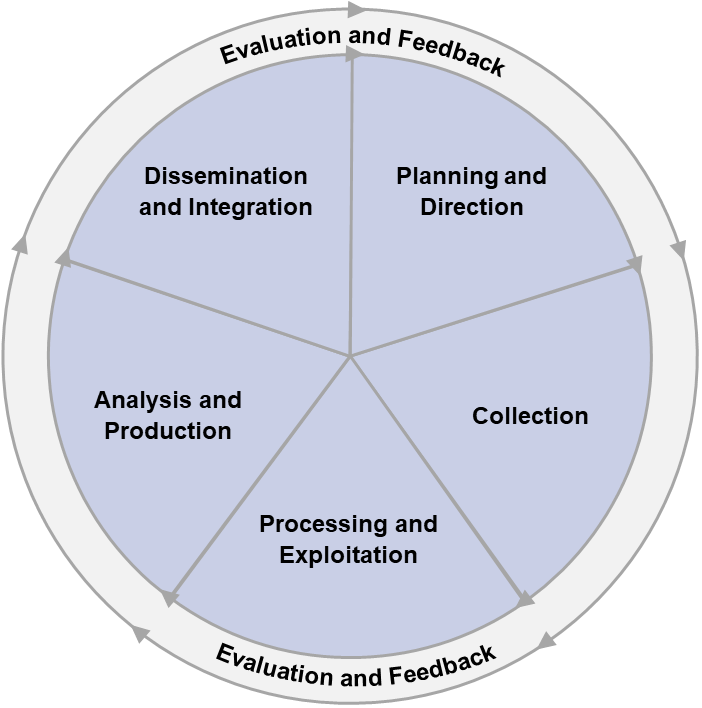
\includegraphics[clip,width=0.9\linewidth]{Intelligence Cycle}
    \caption{Intelligence Cycle, according to \cite{JointChiefsofStaffU.S.Army.2013}}
    \label{fig: intelligence cycle}
\end{figure}

The planning and direction phase combines the identification, definition and prioritization
of the requirements for the cycle. It is also responsible for developing the activities
required to achieve these \cite{DepartmentoftheArmy.2012} and monitoring their implementation
\cite{JointChiefsofStaffU.S.Army.2013, DepartmentoftheArmy.2012}.
The collection phase refers to the gathering of raw data \cite{CentralIntelligenceAgency.1987}.
The core of this phase consists of the iterative repetition of research
\cite{NorthAtlanticTreatyOrganization.2001} to make the query more precise with each run
\cite{PastorGalindo.2020}. The processing and utilization phase involves condensing
these data volumes into valuable and action-relevant information for further processing
\cite{DirectorofNationalIntelligence.2011, JointChiefsofStaffU.S.Army.2013, PastorGalindo.2020, }.
Analysis and production refers to the synthesis of the information obtained into a
user-oriented, timely and accurate intelligence product
\cite{DepartmentoftheArmy.2012, Hwang.2022, NorthAtlanticTreatyOrganization.2001}.
The final phase consists of handing over the finished product to the "customer" in a
usable form \cite{CentralIntelligenceAgency.2023, DepartmentoftheArmy.2012, Williams.2018}.
Evaluation and feedback are not to be regarded as individual phases within the cycle
but take place continuously throughout the entire process. The aim is to achieve progressive optimization
\cite{DirectorofNationalIntelligence.2011, JointChiefsofStaffU.S.Army.2013, NorthAtlanticTreatyOrganization.2001}.

\subsection{Previous Studies}

In the literature, eight previous, publicly accessible literature reviews can be identified
concerning OSINT. In 2017, Dos Passos \cite{DosPassos.2017} showed how big data and data science can
make the decision-making process more useful and effective. Pastor-Galindo et al. then described
the current state of OSINT in 2019 \cite{PastorGalindo.2019} and 2020 \cite{PastorGalindo.2020}
focusing on services and techniques to improve cybersecurity. Moreover, they are also responsible
for the first and only rudimentary mapping of OSINT trends. They observed that OSINT is used in
social opinion and sentiment analysis, cybercrime and organized crime, and cybersecurity and cyberdefence.
Two further literature reviews were published in 2020. García Lozano et al. \cite{GarciaLozano.2020} identified
methods for computer-assisted veracity assessment of public information.
Herrera-Cubides et al. \cite{HerreraCubides.2020} investigated how the production of
research and educational materials in the field of OSINT has developed. They concluded that
the number of publications is lower compared to other trending topics. Finally, in 2021,
Yogish and Krishna \cite{Yogish.2021} explored the state of implementation and use of AI
(Artificial Intelligence) technologies in the context of cybersecurity. The result of this
study showed that Machine Learning (ML), pattern recognition and Natural Language Processing
(NLP) can simplify OSINT in view of increasing data volumes. In the following year, Hwang et al.
\cite{Hwang.2022} investigated security threats and cybercriminality in the context of OSINT misuse.
In 2023, Ghioni et al. \cite{Ghioni.2023} then examined the political, ethical, legal and social implications of
OSINT in conjunction with AI. They discovered that there is still no framework
for addressing these. They also found that third-generation OSINT is still in its early
stages and that human components cannot yet be replaced.

\section{Research Methodology}

The structure of the study is based on the iterative DSRM \cite{Peffers.2007}. It is a theory-based
research paradigm for developing an explicitly applicable solution, in the form of an innovative artifact,
\cite{vomBrocke.2020b}, solving a (practical) problem \cite{Peffers.2007,Hevner.2004}. The model is therefore ideally suited to
create the trend radar. It consists of six successive activities (see Fig. X) \cite{Peffers.2007}.
Moreover, the first three evaluation steps according to Sonnenberg and vom Brocke \cite{Sonnenberg.2012}
were applied to continuously evaluate the design process.

\begin{figure}[h]
    \centering
    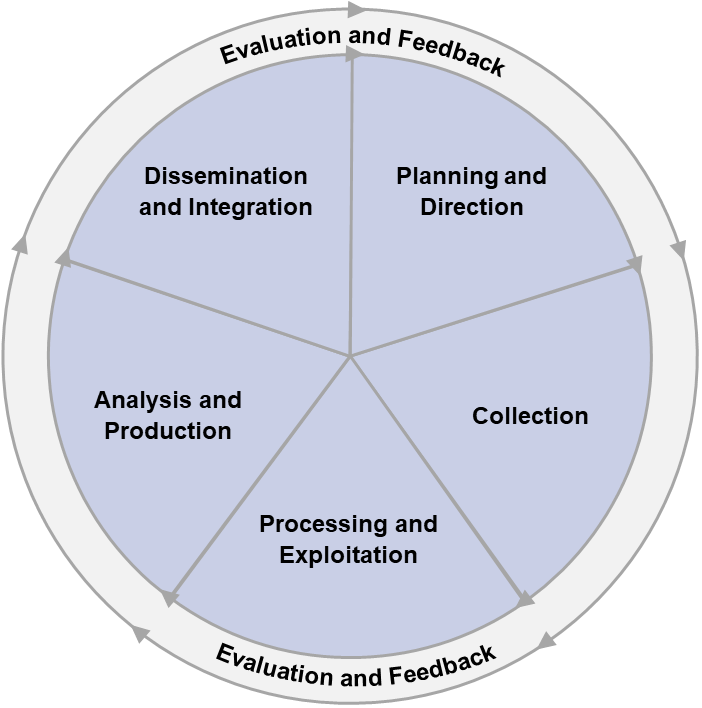
\includegraphics[clip,width=0.9\linewidth]{Intelligence Cycle}
    \caption{Intelligence Cycle, according to \cite{JointChiefsofStaffU.S.Army.2013}}
    \label{fig: intelligence cycle}
\end{figure}


\subsection{Problem Identification and Motivation}

First, the research problem must be defined and the benefits of the solution explained. 
This activity can be found in the chapter Introduction.

\subsection{Design Objectives of the Solution}

The next step entails defining the design objectives of the solution. The
objectives can be divided into two content-related objectives (CO) and
two formal objectives (FO).CO1 requires the trend radar to follow a procedural
structure that reflects the process of generating knowledge from
public information. This will allow a structured mapping of the
identified technologies according to their use. In doing so, any
research gaps that become apparent can be directly assigned to the
respective phase. It will thus be possible to verify if a robust,
autonomous OSINT system exists. As CO2, it was defined that the key
characteristics, in particular the maturity level of the technologies
and their use cases, must be taken into account. The maturity level of
the technologies makes it possible to determine the respective state
of research. Through the use cases the research directions can be
revealed. As FO1, it was determined that the trend radar must follow
a simple structure in order to provide an easy-to-understand knowledge
base for the immediate identification of research gaps. In addition,
the radar should have a high degree of standardization to be
transferable to other intelligence (gathering) disciplines in later
studies. As FO2, it was set out to design the trend radar in an
adaptable and continuously expandable way allowing it to capture the
high field dynamics.

\subsection{Evaluation of the Problem Statement and Design Objectives}

In the theoretical background section, the main definitions and, in
particular, the intelligence cycle, which serves as a basis for the
development of the trend radar ("suitability"), were presented. In
addition, the presentation of previous research work showed that there
is still a lack of comprehensive studies examining OSINT. Both the
relevance of the research question raised and the suitability of the
adopted design objectives are thus underpinned, fulfilling the
evaluation criteria according to Sonnenberg and vom Brocke \cite{Sonnenberg}.

\subsection{Design and Development}

The third activity involves the creation of the artifact. For this
purpose, the relevant literature on OSINT was analyzed by means of a
systematic literature review, following the guidelines of
Cleven et al [47]. To clearly determine the scope of the literature
review, Cooper's taxonomy [48] was used. Subsequently, classification
categories were defined to establish concept matrices, based on the
model of Webster and Watson [24], for systematically analyzing the
researched literature. To achieve a high degree of standardization,
general categories were defined for each phase of the intelligence
cycle. Thereby, the categories of the collection phase differ from
those of the remaining phases, as the data basis is also considered
here. The evaluation and feedback phase was not treated separately due
to its iterative nature.

The following six categories were defined with regard to the survey
phase: "Use case", "Data", "Process", "Technology", "Technology
complexity" and "Maturity level". First of all, the use cases were
used to record the area of application of the technologies. The
category data reveals the composition of the data foundation. Therefore,
it is further subdivided into the data type to record the formats and
the source to show the origin of the data. The third category, the
process, is used to determine the degree of automation or
autonomization of the technologies. For this purpose, the following
four levels were defined: manual, semi-automated, automated,
[Duncheon 2002] fully automated/autonomous
[Billing 1997, Endsley and Kaber 1999]. To improve categorization,
the ten levels of automation
    [Sheridan and Verplank 1978, Parasurama 2000] were additionally used.

The fourth category serves to capture the technologies, according to
Bleck's definition [49], defined as "the totality of material and
immaterial means available for the input, output, conversion,
transmission and storage of information".

The fifth category evaluates the complexity of the technologies
examined. For the collection phase, the three subcategories
"Volume"[53], "Variety" and "Velocity" were used [50-52]. Variety
is further subdivided according to the data structure (structured
    [54], semi-structured and unstructured [55,56]) [53]. Velocity,
is further subdivided into the levels "Batch" [58], "Near Real-Time"
[59,60] and "Real-Time" [59].

The sixth category reflects the maturity level of the technologies used.
For this purpose, the three macro-maturity phases of the German Federal
Trend Radar are used: the innovation phase, the prototype phase and
the market establishment phase [61].

For the remaining phases of the intelligence cycle, the categories use
case, process, technology, technology complexity and maturity level
were likewise defined. However, the complexity within the remaining
phases is measured on the basis of the underlying analysis, in
ascending order: descriptive analysis, diagnostic analysis, predictive
analysis through to prescriptive analysis [63,64].

After defining the classification criteria, the literature research
was carried out (see Fig. 15). For this, a search string based on
general terms for the highest possible number of hits was determined.
The string was then applied to the four databases "Web of Science",
"IEEE Xplore", "ACM Digital Library" and "arXiv". The search results
were restricted to publications in German or English. Only studies
with full access were considered. As the number of publications
increased significantly between 2020 and 2023, the period was reduced
to these years to ensure the most up-to-date coverage possible.
The studies were downloaded on 05.06.2023 (see Appendix D.B). The
SQR3 method [65] was applied for the systematic analysis and further
delimitation. Altogether 60 studies were categorized following this
procedure.

For categorization, a dedicated Excel spreadsheet was created for each
Intelligence Cycle phase and the OSINT technologies and their
characteristics methodically recorded [24,47]. The identified
technologies were then grouped according to related technologies in an
additional Excel column to enable the clear final illustration in the
trend radar (see Repository X). Afterwards, the categorization was
reviewed by using a "Python" script (see Appendix A). The script
queries the occurrence of predefined keywords in the included papers.
If a deviation was found, the study in question was analyzed again
(see review matrix X). Finally, the trend radar was created on the
basis of the concept matrices.

\subsection{Evaluation of the Design Specifications}

The intelligence cycles as the basis of the trend radar provides a
structured overview ("clarity") (Breakspear, 2013, p. 689 f.). This
meets the requirement of an intuitively understandable illustration
("under-standability") for ensuring a simple extraction ("simplicity")
of technologies and research gaps. Furthermore, the other intelligence
disciplines are also derived from the cycle, which enables a later
application to these ("applicability"). In addition, by aligning the
architecture of the radar with the federal government's trend radar
(cf. Stich et al., 2022, p. 11 f.), a proven, robust, user-friendly
design ("userfriendliness") with an appropriate level of detail
("level of detail") is used. Moreover, with the concept matrices, a
template is used to constantly update the radar in order to reflect
the highly dynamic nature of the research topic. Particular attention
was paid to the general validity of the categories in order to achieve
the highest possible degree of standardization ("commonality"). The
categorization was also reviewed using the Python script ("internal
consistency"). The decisive evaluation criteria, according to
Sonnenberg and vom Brocke (2012, p. 13), are thus fulfilled.

\subsection{Demonstration}

Next, the trend radar was demonstrated in the context of guided,
systematizing expert interviews. Especially in less structured and
sparsely linked subject areas, the method enables dense data collection
    [66,25]. Additionally, it is suitable in cases where access to the
social field is limited [66,26]. The execution thereby follows the
concepts of Bogner et al [25], Meuser and Nagel [67] and Gläser and
Laudel [26].

The experts (see Tab. 1) were selected according to the method of
theoretical sampling [68,69]. It was specified that only experts in
Germany should be interviewed in order to validate the trends in this
country. Furthermore, it was determined that at least one expert each
from a security authority, the established security industry and a
start-up would be selected in order to capture different points of
view. Following Meuser and Nagel [70], an expert was considered to be
someone with a knowledge advantage in the specific area of interest.
A "prestigious" company position is they regarded as a reliable
guarantee that the respondents possess research-relevant knowledge [72].

The qualitative data collection that followed was carried out using
semi-structured interviews. These are particularly suitable for
revealing the underlying relationships of a theory [25]. The
questionnaire used is based on the structure of the Intelligence Cycle.
At the beginning of the interview, the subjects were introduced to the
trend radar. In order to compare this theoretical construct with the
practical experience of the participants, higher-level, open questions
were asked for each phase. These questions reduce the influence of
subjectivity [73]. In order to direct the conversation flow in a
targeted manner, the superordinate questions are supplemented by
exploratory questions [73]. At the third level, these questions are
complemented by specific closed questions for targeted follow-up
queries [73]. The interviews were held within a time frame of up to
one hour, with a maximum of three main questions for each section
 [25] (see Respository X). The questionnaire was pilot-tested with a
domain expert. The expert interviews were conducted online via
platforms with video chat functions.

\subsection{Evaluation of the First Instance of the Trend Radar}

The demonstration of the trend radar confirmed its intuitive
comprehensibility ("ease of use"). It was furthermore perceived by the
practitioners as a useful tool for providing an overview of OSINT
technologies ("effectiveness"). In addition, they confirmed its
completeness ("completeness") and internal consistency ("consistency")
(cf. expert E1, 14.08.2023; expert E3, 28.07.2023; expert E4,
02.08.2023). The design of the trend radar thus proved to be a
suitable instrument for identifying research gaps in theory-practice
comparisons and for serving as a guideline to practitioners
("fidelity with real world phenomenon"). The essential evaluation
criteria, according to Sonnenberg and vom Brocke (2012, pp. 15-18),
are thus demonstrably fulfilled in practice.

\subsection{Evaluation}

The evaluation was carried out using a qualitative data analysis
according to Gläser and Laudel [26]. The aim of this is to extract,
synthesize and structure the information contained in the interviews
on the basis of a predefined search grid. This enables the targeted
extraction and summarization of relevant, cross-interview information
according to a "top-down approach" [26,25]. The established category
system was applied for this purpose.

First, the recorded interviews were transcribed. Second, the software
MAXQDA [75] was used for the subsequent categorization and analysis.
The categorization system was therefor established within MAXQDA
(see repository X). The categories of the first level correspond to
the individual phases of the intelligence cycle. The categories of the
second level allow a classification of whether the experts express
themselves in support of or in contradiction to the theory. The
categories of the third level reflect the identified use cases.
As many of the experts' statements were of a general nature, the
category "General statements" was added at this level. The categories
of the fourth level reflect the individual technologies classified
under them. Altogether, 257 statements from the experts were assigned
to corresponding categories by this method. Examples of the coding
procedure can be found in (Table 3).

\subsection{Communication}

The research results are communicated in the form of this study.
A new iteration, proceeding from this chapter, is therefore not
carried out.

\section{Graphics/Images}

All images must be embedded in your document or included with your submission as individual source files. The type of graphics you include will affect the quality and size of your paper on the electronic document disc. In general, the use of vector graphics such as those produced by most presentation and drawing packages can be used without concern and is encouraged.

\begin{itemize}
    \item Resolution: 600 dpi
    \item Color Images: Bicubic Downsampling at 300dpi
    \item Compression for Color Images: JPEG/Medium Quality
    \item Grayscale Images: Bicubic Downsampling at 300dpi
    \item Compression for Grayscale Images: JPEG/Medium Quality
    \item Monochrome Images: Bicubic Downsampling at 600dpi
    \item Compression for Monochrome Images: CCITT Group 4
\end{itemize}

If your paper contains many large images they will be down-sampled to reduce their size during the conversion process.  However, the automated process used will not always produce the best image, and you are encouraged to perform this yourself on an image by image basis. The use of bitmapped images such as those produced when a photograph is scanned requires significant storage space and must be used with care.

\section{Main text}

Type your main text in 10-point Times, single-spaced. Do not use double-spacing. All paragraphs should be indented 1/4 inch (approximately 0.5 cm).  Be sure your text is fully justified—that is, flush left and flush right. Please do not place any additional blank lines between paragraphs. \\
\textbf{Figure and table captions} should be 9-point boldface Helvetica (or a similar sans-serif font).  Callouts should be 9-point non-boldface Helvetica. Initially capitalize only the first word of each figure caption and table title. Figures and tables must be numbered separately. For example: ``Figure 1. Database contexts'', ``Table 1. Input data''. Figure captions are to be centered below the figures. Table titles are to be centered above the tables.

% For one-column wide figures use
\begin{figure}[thb]
    % Use the relevant command to insert your figure file.
    % For example, with the graphicx package use
    \centering
    
\includegraphics[trim={3cm 3cm 3cm 3cm}, clip,width=0.9\linewidth]{sample-image}
    % figure caption is below the figure
    \caption{Sample figure with caption.}
    \label{fig: sample-figure}       % Give a unique label
\end{figure}

\section{First-order headings}

For example, “1. Introduction”, should be Times 12-point boldface, initially capitalized, flush left, with one 12-point blank line before, and one blank line after. Use a period (“.”) after the heading number, not a colon.

\subsection{Second-order headings}

As in this heading, they should be Times 11-point boldface, initially capitalized, flush left, with one blank line before, and one after.

\subsubsection{Third-order headings. }

Third-order headings, as in this paragraph, are discouraged. However, if you must use them, use 10-point Times, boldface, initially capitalized, flush left, followed by a period and your text on the same line.

\section{Footnotes}

Use footnotes sparingly and place them at the bottom of the column on the page on which they are referenced. Use Times New Roman 8-point type, single-spaced. To help your readers, try to avoid using footnotes altogether and include necessary peripheral observations in the text (within parentheses, if you prefer, as in this sentence).
asdöfj
% Fonts specification --- not shown as it doesn't exist in the Word document either. 

%\section{Fonts}

%A summary of fonts is provided in Table \ref{tab: fonts}. 

%\begin{table}[thb]
%\centering
%\caption{\label{font-table} Font guide. \vskip 3pt }
%\label{tab: fonts}
%\begin{tabular}{l|rl}
%\hline \bf Type of Text & \bf Font Size & \bf Style \\ \hline
%paper title & 14 pt &  \bf bold \\
%authors & 10 pt &  \underline{email} underlined \\
%abstract title & 12 pt &  \bf bold\\
%abstract text & 10 pt &  \it italic\\
%section titles & 12 pt & \bf bold \\
%subsection titles & 11 pt & \bf bold \\
%document text & 10 pt  & \\
%captions & 9 pt & \sansserifformat{\captionsize sans-serif, \bf bold} \\
%bibliography & 9 pt & \\
%footnotes & 8 pt & \\
%\hline
%\end{tabular}
%\end{table}


\section{References}


%Bibliography 

\bibliographystyle{ieeetr}
\bibliography{references}




\end{document}
